\chapter{實驗設計與結果}
\label{c:experiment}

在本章中,我們將在不同工作量下評估
以不同資料結構分別實作的持久化 LRU 性能。

\section{實驗環境}
實驗均在以下環境中進行

\begin{itemize}
\item CPU: AMD Ryzen 7 2700X (8 核心 16 執行緒、3.6 GHz、32K L1d 快取、64k L1i 快取、512K L2 快取、8M L3 快取)
\item 記憶體: DDR4 64 GB
\item 作業系統:Linux manjaro 4.19.36-1-MANJARO x86\_64
\item 編譯器: GCC 9.1.0
\end{itemize}

\section{資料結構}

我們以 C++ 17 撰寫了三種資料結構:

\begin{itemize}
\item 雜湊 + 雙向鏈表(3.4 節),每次建立新版本都會完全複製一次自己
\item 持久化雜湊 + 持久化紅黑樹(3.4.1 節)
\item 持久化雜湊 + 持久化順序樹(3.4.2 節)
\end{itemize}

由於要模擬的是區塊鏈,所以所有的工作量都以區塊為單位,
而一個區塊會包含多個 get/put 。為此,以上實作的持久化資料結構都支援了 transient \cite{puente2017persistence},
也就是說,資料結構不需要對每一個 get/put 都生成一個新版本,而是暫時生成一個版本,
在其上進行多個操作,再將它固定為不可變的,
由於減少了大量的中間狀態,此舉能夠大幅提升效能。

函式庫使用方面,雜湊直接使用了 C++ 標準庫的 unordered\_map ,
持久化雜湊則採用了著名的 C++ 不可變資料結構函式庫 \href{https://sinusoid.es/immer/}{immer} ,
其餘的雙向鏈表、持久化紅黑樹、持久化順序樹則自行撰寫。

往後,我們會以雙向鏈表、紅黑樹、順序樹來簡稱這三個複合資料結構。

\section{速度}

\subsection{工作量}
我們採用一個簡單的模型來模擬區塊生成,網路中有 n 個節點,
每個節點都會針對自己認定的最高區塊(亦即,它所認同的最長鏈的頂端)挖礦,初始時,
每個節點的最高區塊都是創世區塊(genesis block)。其後,有若干回合,
每個回合中,每個節點有一定概率會挖出新區塊。若它沒有挖到,
則會投奔其他節點挖出的同最高區塊的後繼區塊,若該最高區塊沒有任何後繼區塊,
則會隨機投奔其他最長鏈。若沒有任何節點挖到礦,就將同樣的過程再來一次。

在所有的工作量中,都是假定網路中有 10 個節點、每個節點在一個回合內挖到礦的機率是十分之一,
並且在挖出 1000 個區塊之後停止。在此設定下,同個高度大約會有 1.5 個區塊。

從 \href{https://etherscan.io/chart/gaslimit}{etherscan} 可以得知,
以太坊現今的 gas limit 大約是一千萬,而一筆交易的 gas 費用為 21000 ,
一個區塊大約可以包含 500 左右的交易。因此工作量的一個區塊的 get/put 指令數量設定為 500 。

此外,還有一項參數是 get/put 的佔比,對於一般的以太坊交易而言,
每次的付款都會導致賬戶的狀態改變,然而智能合約的情形就不一定,
因此 get, put 兩種指令都有可能出現,以下若無額外說明,put 都占 50\% (get 佔另外 50\%)。

在開始任何一項工作前,我們都會先將整份快取裝滿,若非如此,當快取大小設定太大時,
需要很長一段時間才能將它裝滿,快取未滿時的狀態並非我們關注的,因為區塊鏈動輒幾百萬個區塊,
極大部分時間,快取都是裝滿的。

\subsection{調整快取大小}

第一項實驗將快取命中率固定在 50\% ,調節快取的大小(鍵值對的數量)。

\begin{figure}[h!]
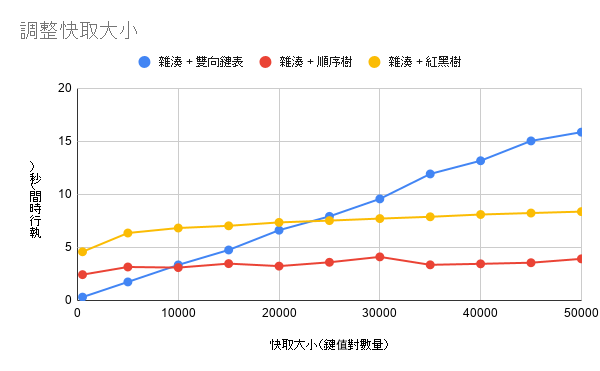
\includegraphics[width=\textwidth]{調整快取大小}
\caption{調整快取大小}
\end{figure}

所畫出的折線圖 4.1,可以大略看出,雙向鏈表的所耗費的時間基本上正比於快取的大小,
顯見雙向鏈表的主要消耗在於複製,快取有多大,每次區塊更新,所要複製的量就有多大。

紅黑樹和順序樹的成長曲線就十分平緩($O(\log n)$),而順序樹的常數又小於紅黑樹。
注意到順序樹的折線中,相較紅黑樹的穩定增長,是有所震盪的,
這跟順序樹的葉子數量是 $2 + \lfloor \log_2 n \rfloor$ 有關,它的葉子數量更加離散,
當快取大小達到 $2^k$ 次方時,就會往上翻倍,此時就會影響效能,導致震盪。

\subsection{調整快取命中率}

將快取大小定為 30000 ,調整命中率 。

\begin{figure}[h!]
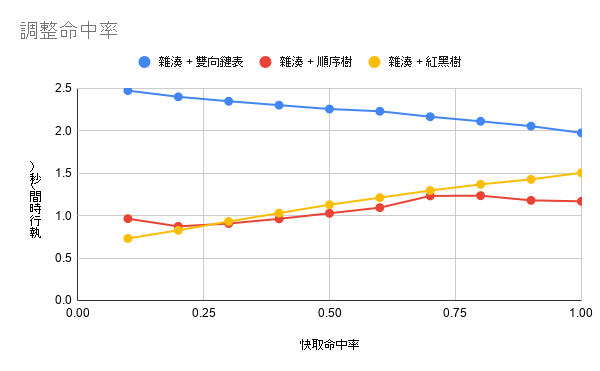
\includegraphics[width=\textwidth]{調整命中率}
\caption{調整命中率}
\end{figure}

圖 4.2 中可見,命中率對雙向鏈表並沒有什麼影響,因為它的主要消耗來自於複製,
快取命中之後所有做的事情只是搬動幾個指針,不花什麼時間。
而紅黑樹、順序樹的耗時都會隨命中率提高而有所上升,
因為它們主要的耗時來自於路徑複製,命中越多,需要複製、創建的分支也就越多。

\subsection{調整 put 比例}

將快取大小定為 30000 ,命中率設為 1.0 ,調整 put 佔兩種指令的比例。從圖 4.3 可見基本不影響效能。

\begin{figure}[h!]
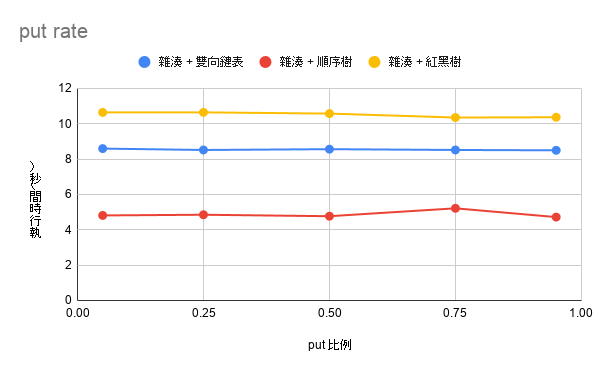
\includegraphics[width=\textwidth]{put_rate}
\caption{調整 put 比例}
\end{figure}

% \subsection{記憶體用量}

\subsection{總結}

實驗驗證了順序樹、紅黑樹較低的時空間複雜度,在快取大小增大到一定程度後,
表現上顯著領先總是複製自身的雙向鏈表。

同時,由於順序樹相較於紅黑樹,無需維護節點顏色,以及判斷各種旋轉規則,
在執行速度上有一定的優勢。